\documentclass[12pt]{beamer}
\usepackage[utf8x]{inputenc}
\usepackage{ucs}
\usepackage{amsmath}
\usepackage{amsfonts}
\usepackage{amssymb}
\usepackage{graphicx}
\mode<presentation>{}
\setbeamertemplate{footline}[frame number]{}
\setbeamertemplate{navigation symbols}{}

\AtBeginSection[]
  {
    \ifnum \value{framenumber}>0
      \begin{frame}<beamer>
      \frametitle{Outline}
      \tableofcontents[currentsection]
      \end{frame}
    \else
    \fi
  }

\author{Mikhail Shugay, PhD}
\title{Immune repertoire forensics}
\subtitle{A RepSeq data analysis tutorial}
\institute[Skoltech]{\texttt {Skoltech, MA03172 course [Term 2, 2017-2018]}}
\date{December 1, 2017}

\begin{document}

\maketitle

\section{Introduction}
\begin{frame}{T-cell receptor}
\begin{columns}
\column{0.55\textwidth}
\textbf{T-cell:APC contact}\\~\

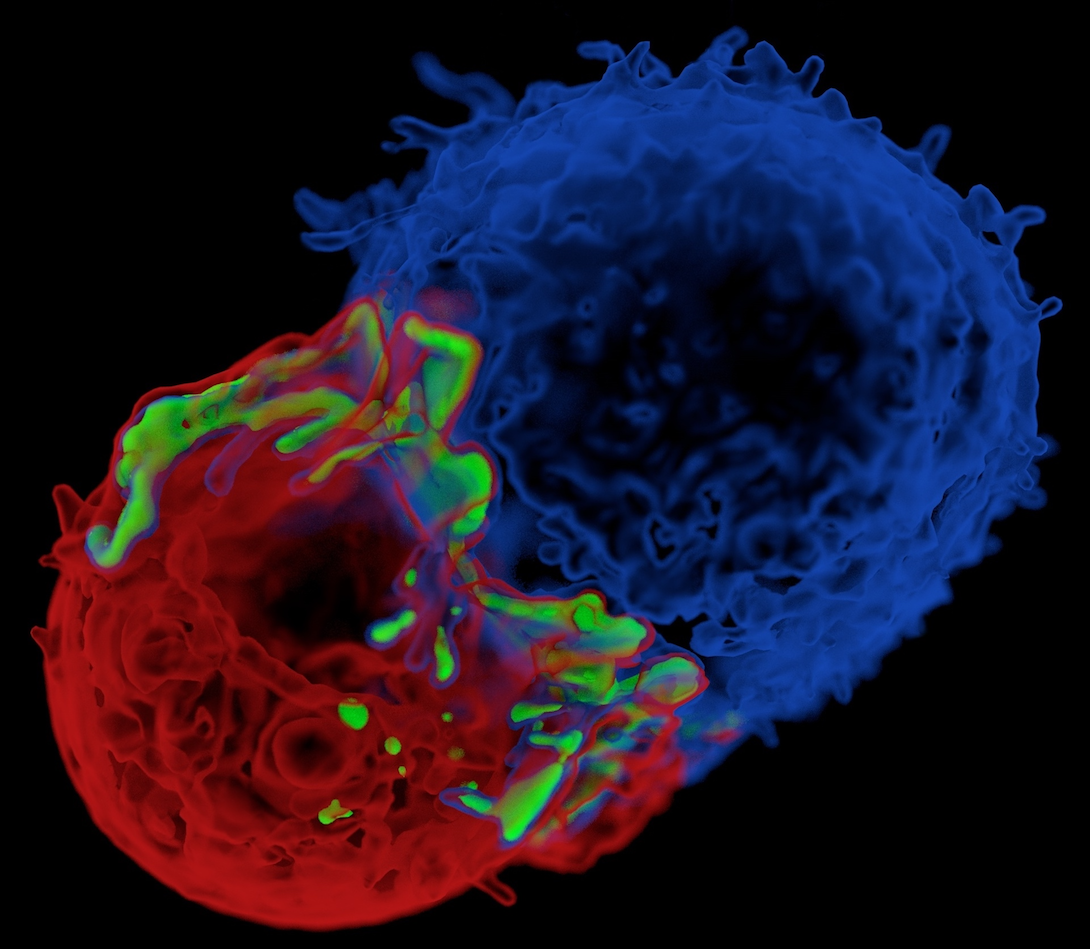
\includegraphics[scale=0.13]{p1}\\~\

From James and Vale, Nature 2012, https://valelab.ucsf.edu/images/
\pause
\column{0.45\textwidth}
\textbf{TCR:pMHC structure}\\~\

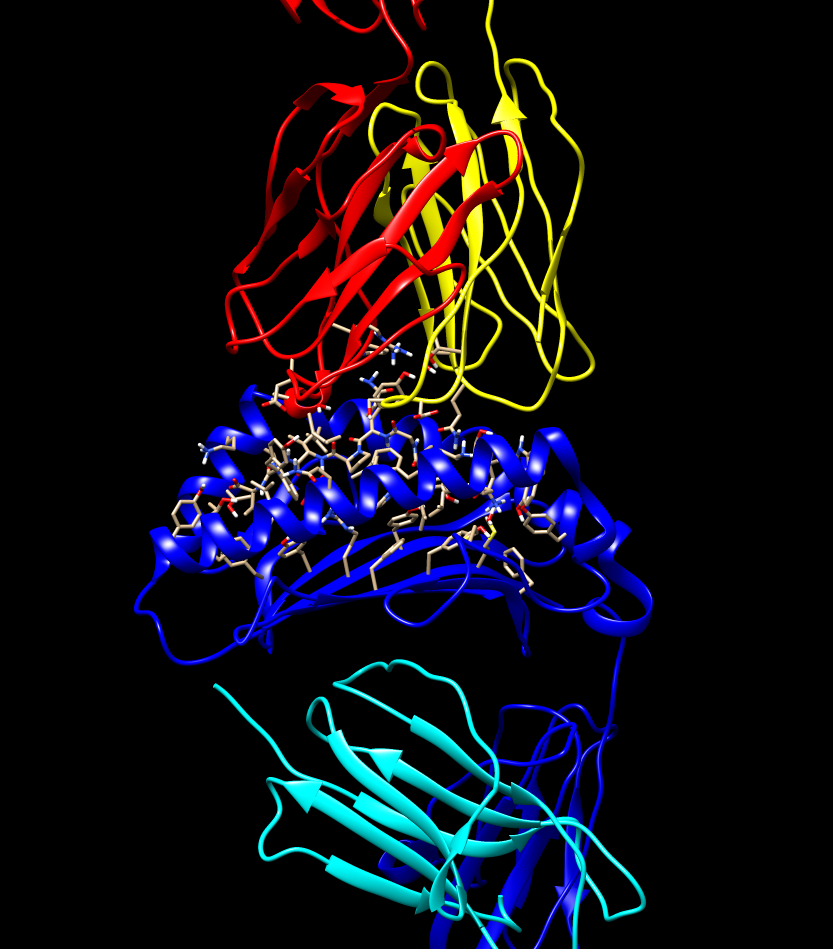
\includegraphics[scale=0.13]{p2}\\~\

PDB:1ao7, rendered using UCSF chimera, colored by chain

\end{columns}
\end{frame}

\begin{frame}{VDJ rearrangement}
An example schema for TCR$\beta$ locus
\begin{center}
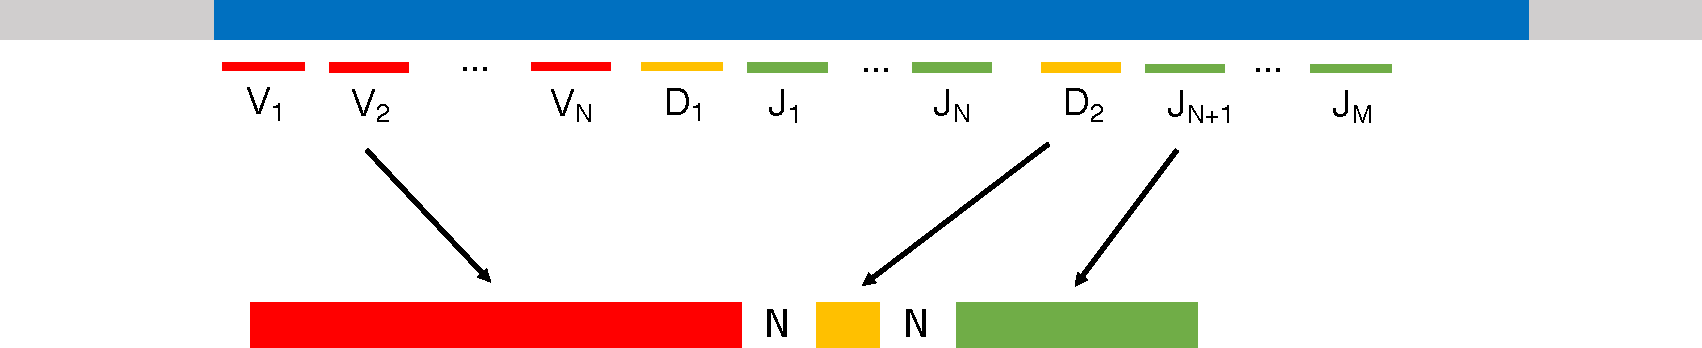
\includegraphics[width=\textwidth]{p3}
\end{center}
Variable, Diversity and Joining are chosen at random, V-D and D-J junctions are filled with non-template N bases. \\~\

\pause
VDJ rearrangement mechanism can be efficiently recaptured with a probabilistic model [\texttt{Murugan et al. PNAS 2012}]
\begin{equation*}
\begin{split}
P\left(\sigma\right) &= P(V)P(D,J) \\
 &\times P(\#del_V|V)P(\#del_J|J)P(\#del_{D5},\#del_{D3}|D) \\
 &\times P(\#ins_{VD})P(\#ins_{DJ})\prod_{i \in ins_{VD}} P(b_i|b_{i-1})\prod_{i \in ins_{DJ}} P(b_i|b_{i+1})
\end{split}
\end{equation*}
\end{frame}

\begin{frame}{TCR regions}
A TCR chains consists of the following regions:
\begin{center}
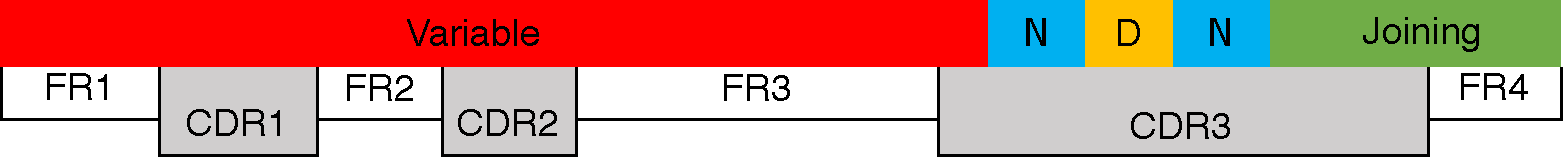
\includegraphics[width=\textwidth]{p4}
\end{center}
In total there are four framework (FRs) and three complementarity determining regions/loops (CDRs). \\~\

\pause
The likely functions of these regions are:
\begin{itemize}
\item FR regions maintain TCR secondary structure and (possibly) play role in MHC binding
\item CDR1,2 are germline encoded and play role in antigen recognition, as well as (possibly) MHC binding
\item CDR3 plays a major role in antigen recognition and is extremely variable
\end{itemize}
\end{frame}

\begin{frame}{TCR repertoire sequencing}
\begin{center}
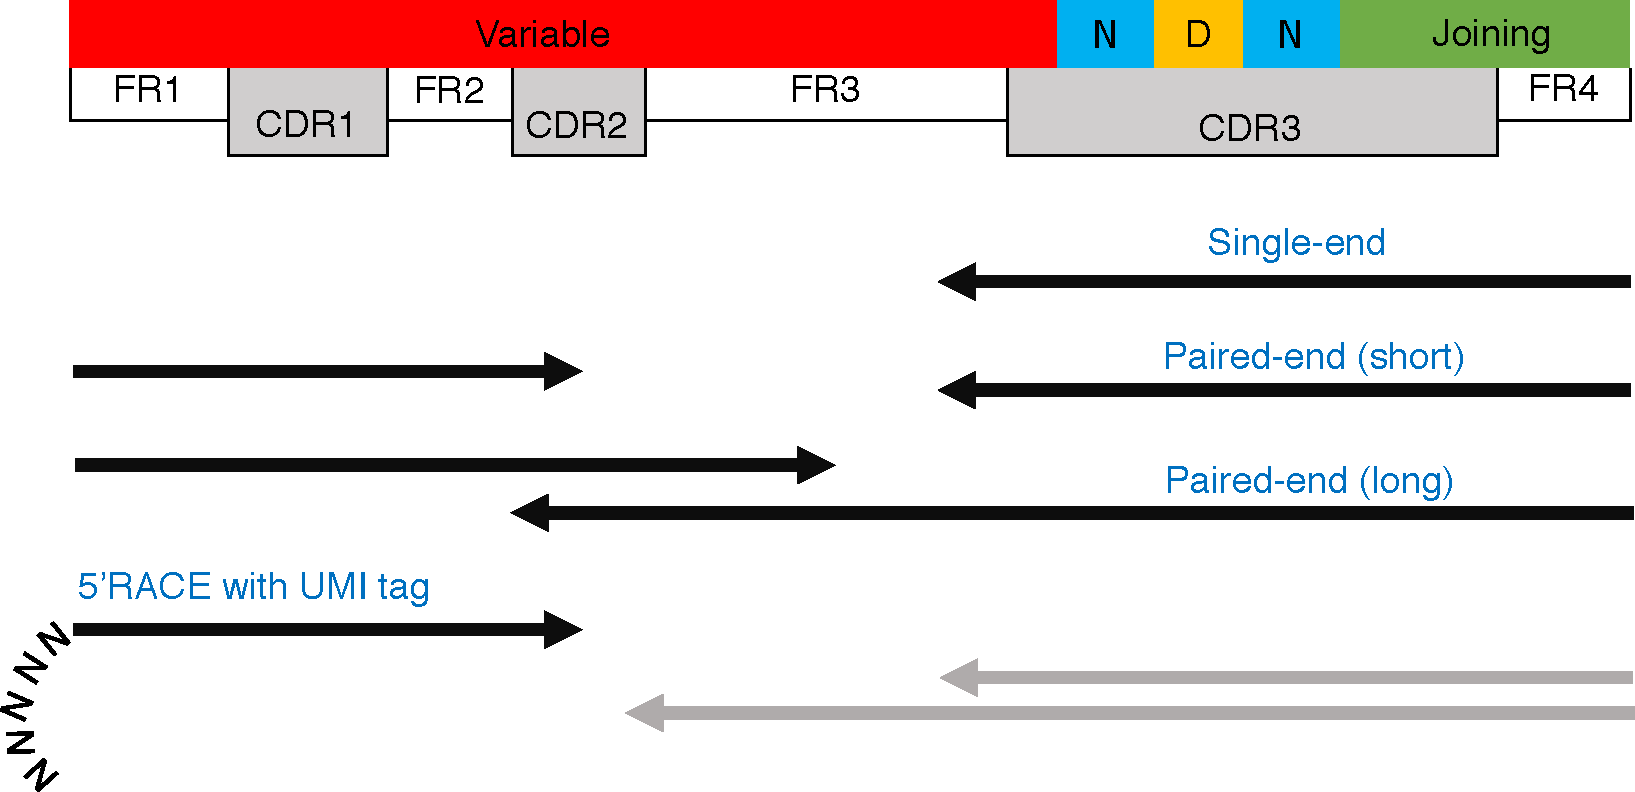
\includegraphics[width=\textwidth]{p5}
\end{center}
\end{frame}

\begin{frame}{An example of a RepSeq dataset}
After all pre-processing steps:
\begin{itemize}
\item Read grooming (filtering, etc)
\item UMI-based assembly (for molecular barcoded data)
\item V-D-J mapping and clonotype assembly\\~\
\end{itemize}

\pause
We finally get clonotype frequency tables that look like
\begin{center}
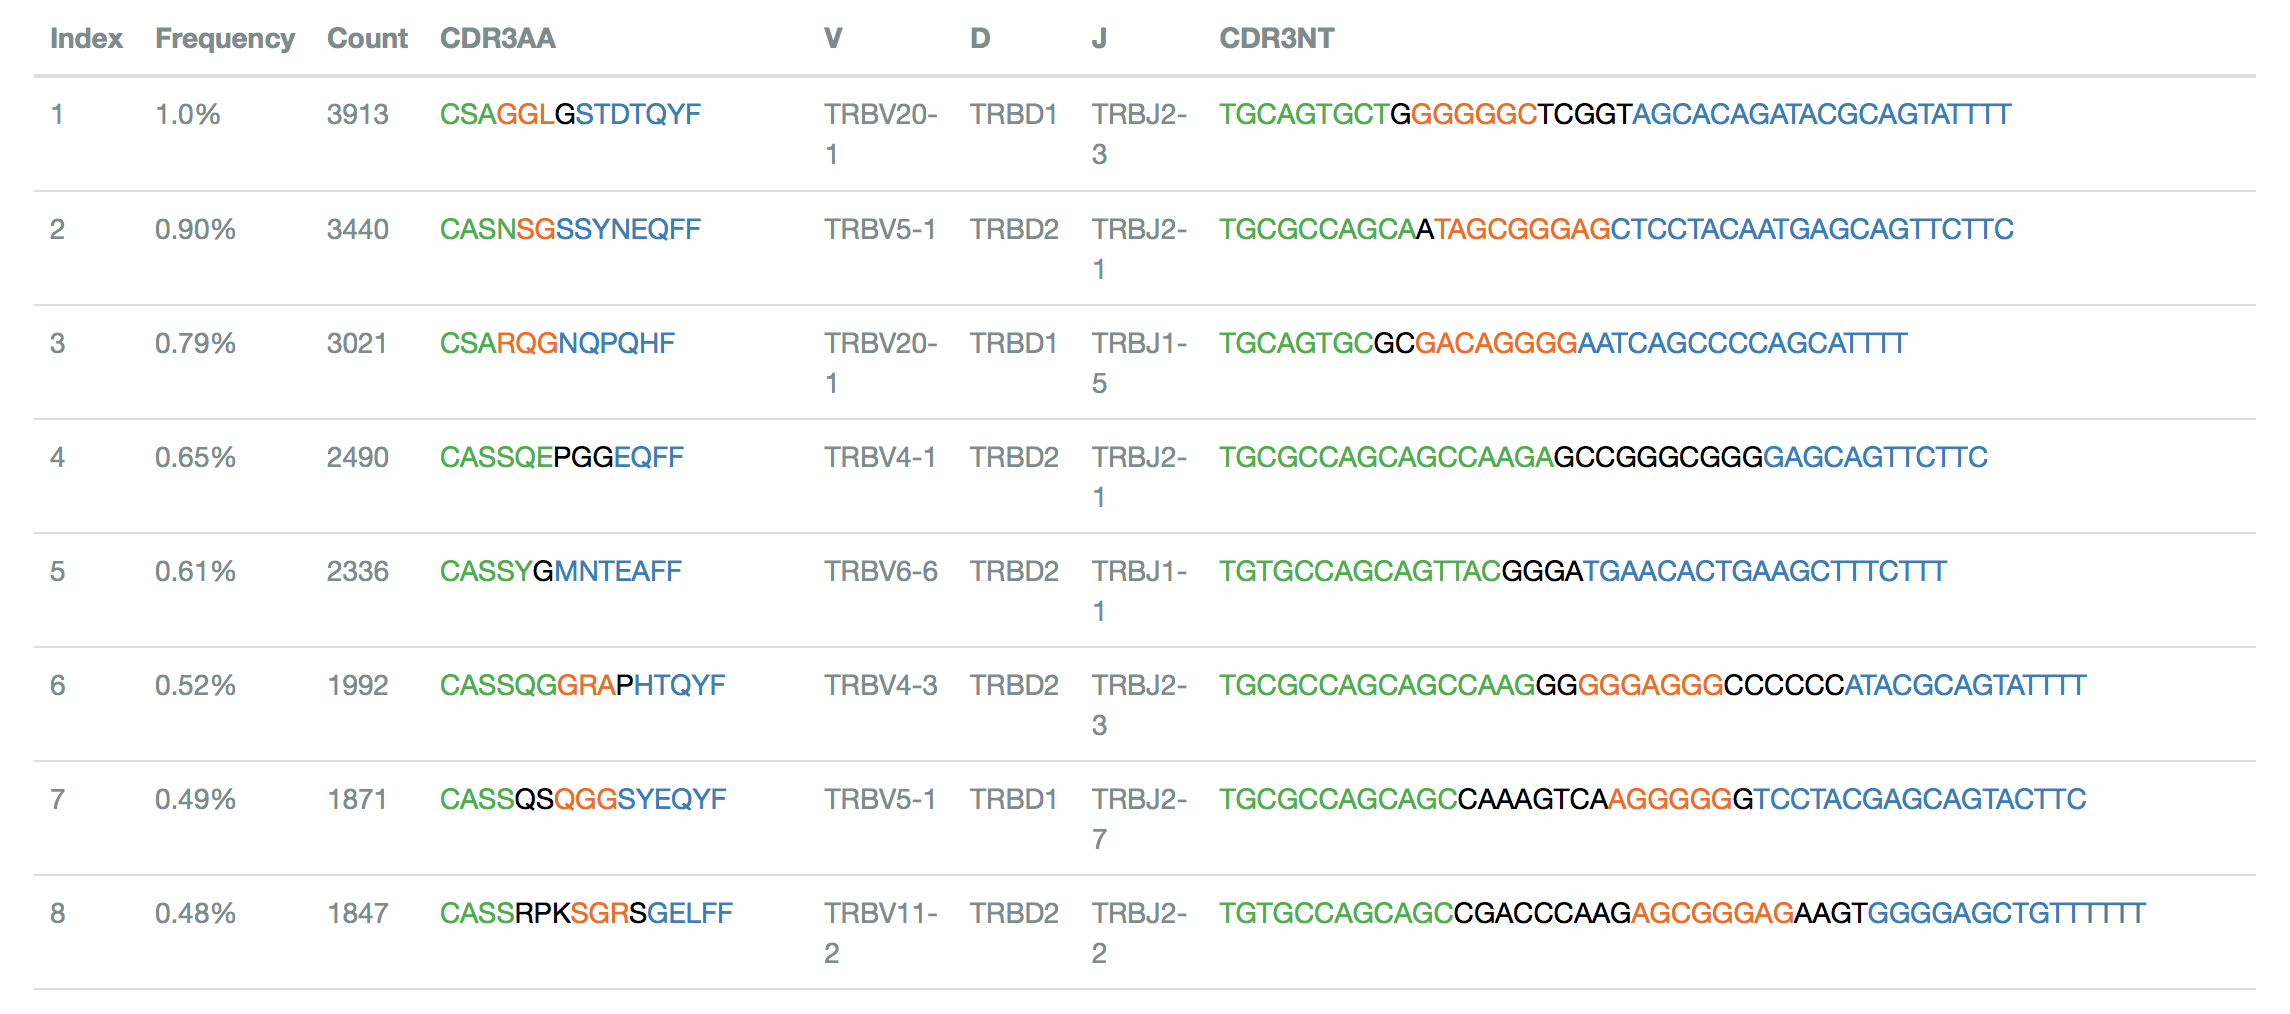
\includegraphics[width=\textwidth]{p6}
\end{center}
\end{frame}

\section{Getting started}

\begin{frame}{Downloading data}
Navigate to \url{https://github.com/antigenomics/repseq-forensics-tutorial} and download the data + code bundle as zip
\begin{center}
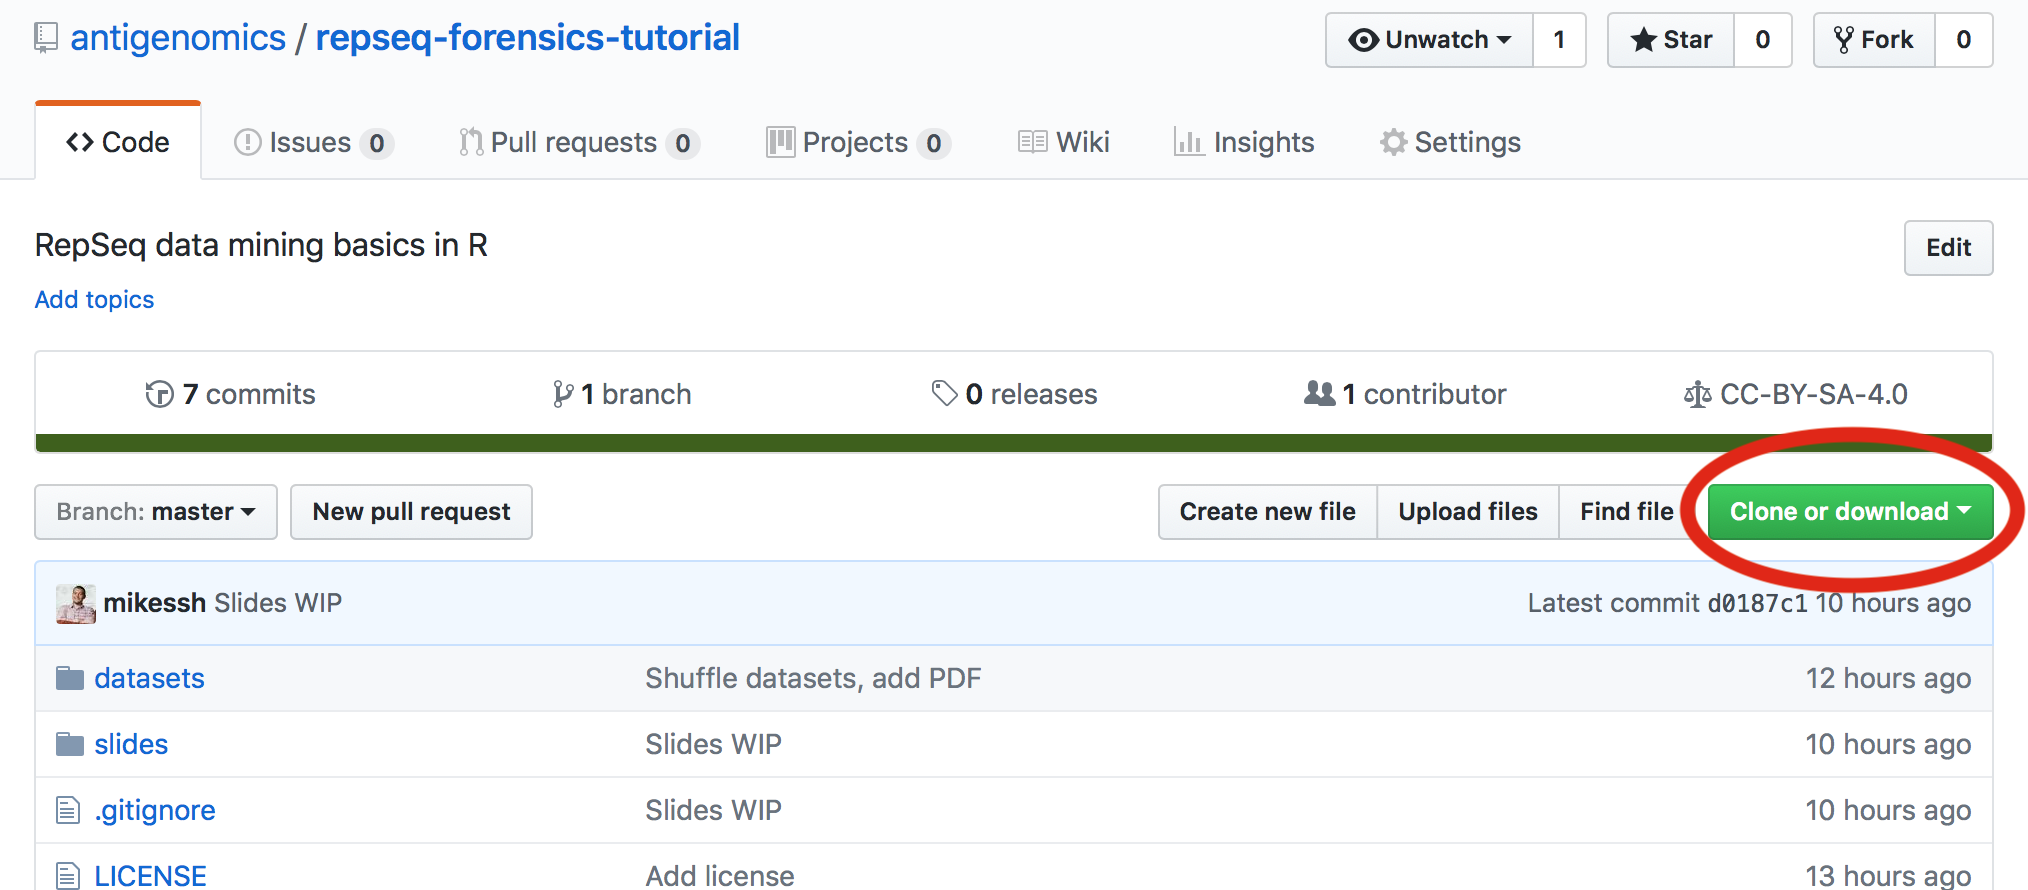
\includegraphics[width=\textwidth]{p7}
\end{center}
\end{frame}

\begin{frame}{Executing R code}
Open the \texttt{tutorial.Rmd} in RStudio, it can be found in the root folder of the bundle.
\begin{center}
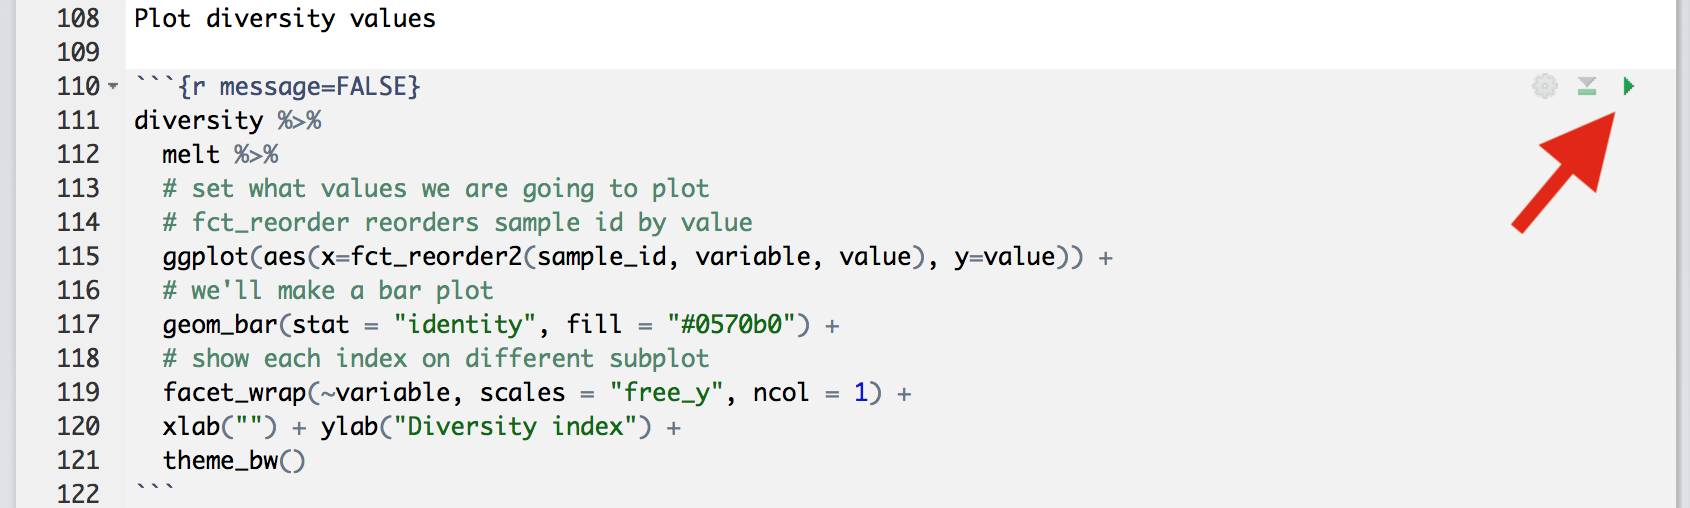
\includegraphics[width=\textwidth]{p8}
\end{center}
\end{frame}

\begin{frame}{Executing R code}
\begin{center}
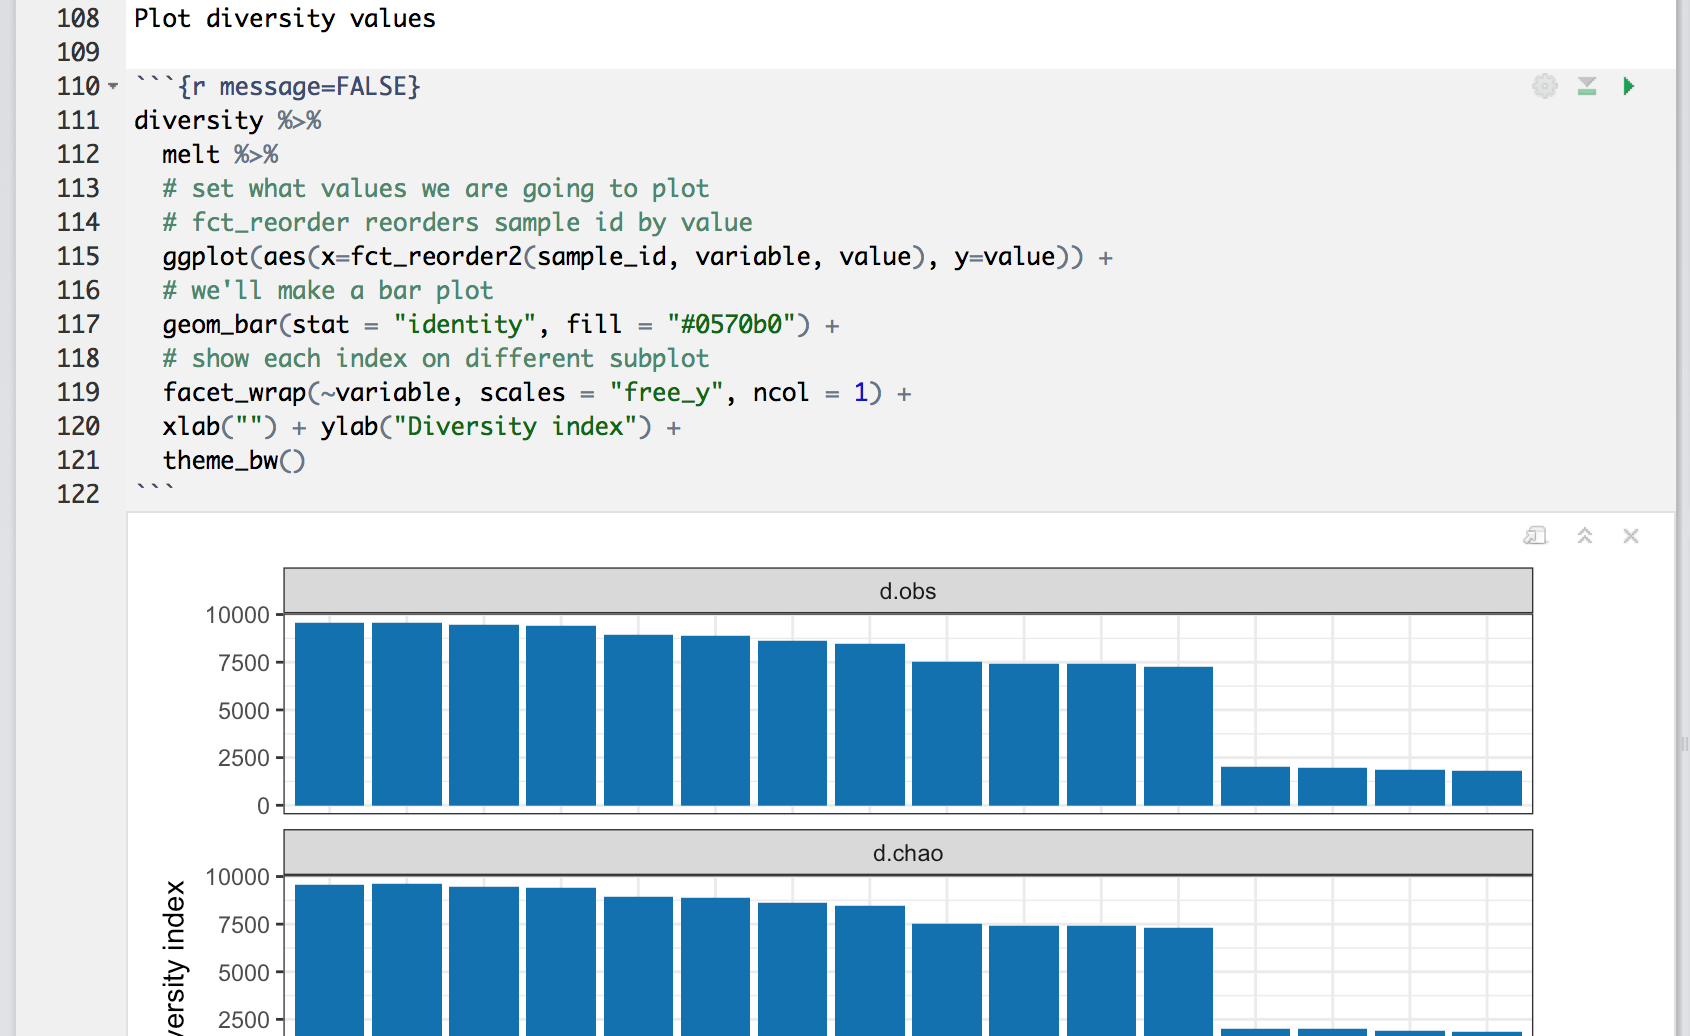
\includegraphics[width=\textwidth]{p9}
\end{center}
\end{frame}

\section{Interactive part}

\begin{frame}{Interactive part}
\begin{center}
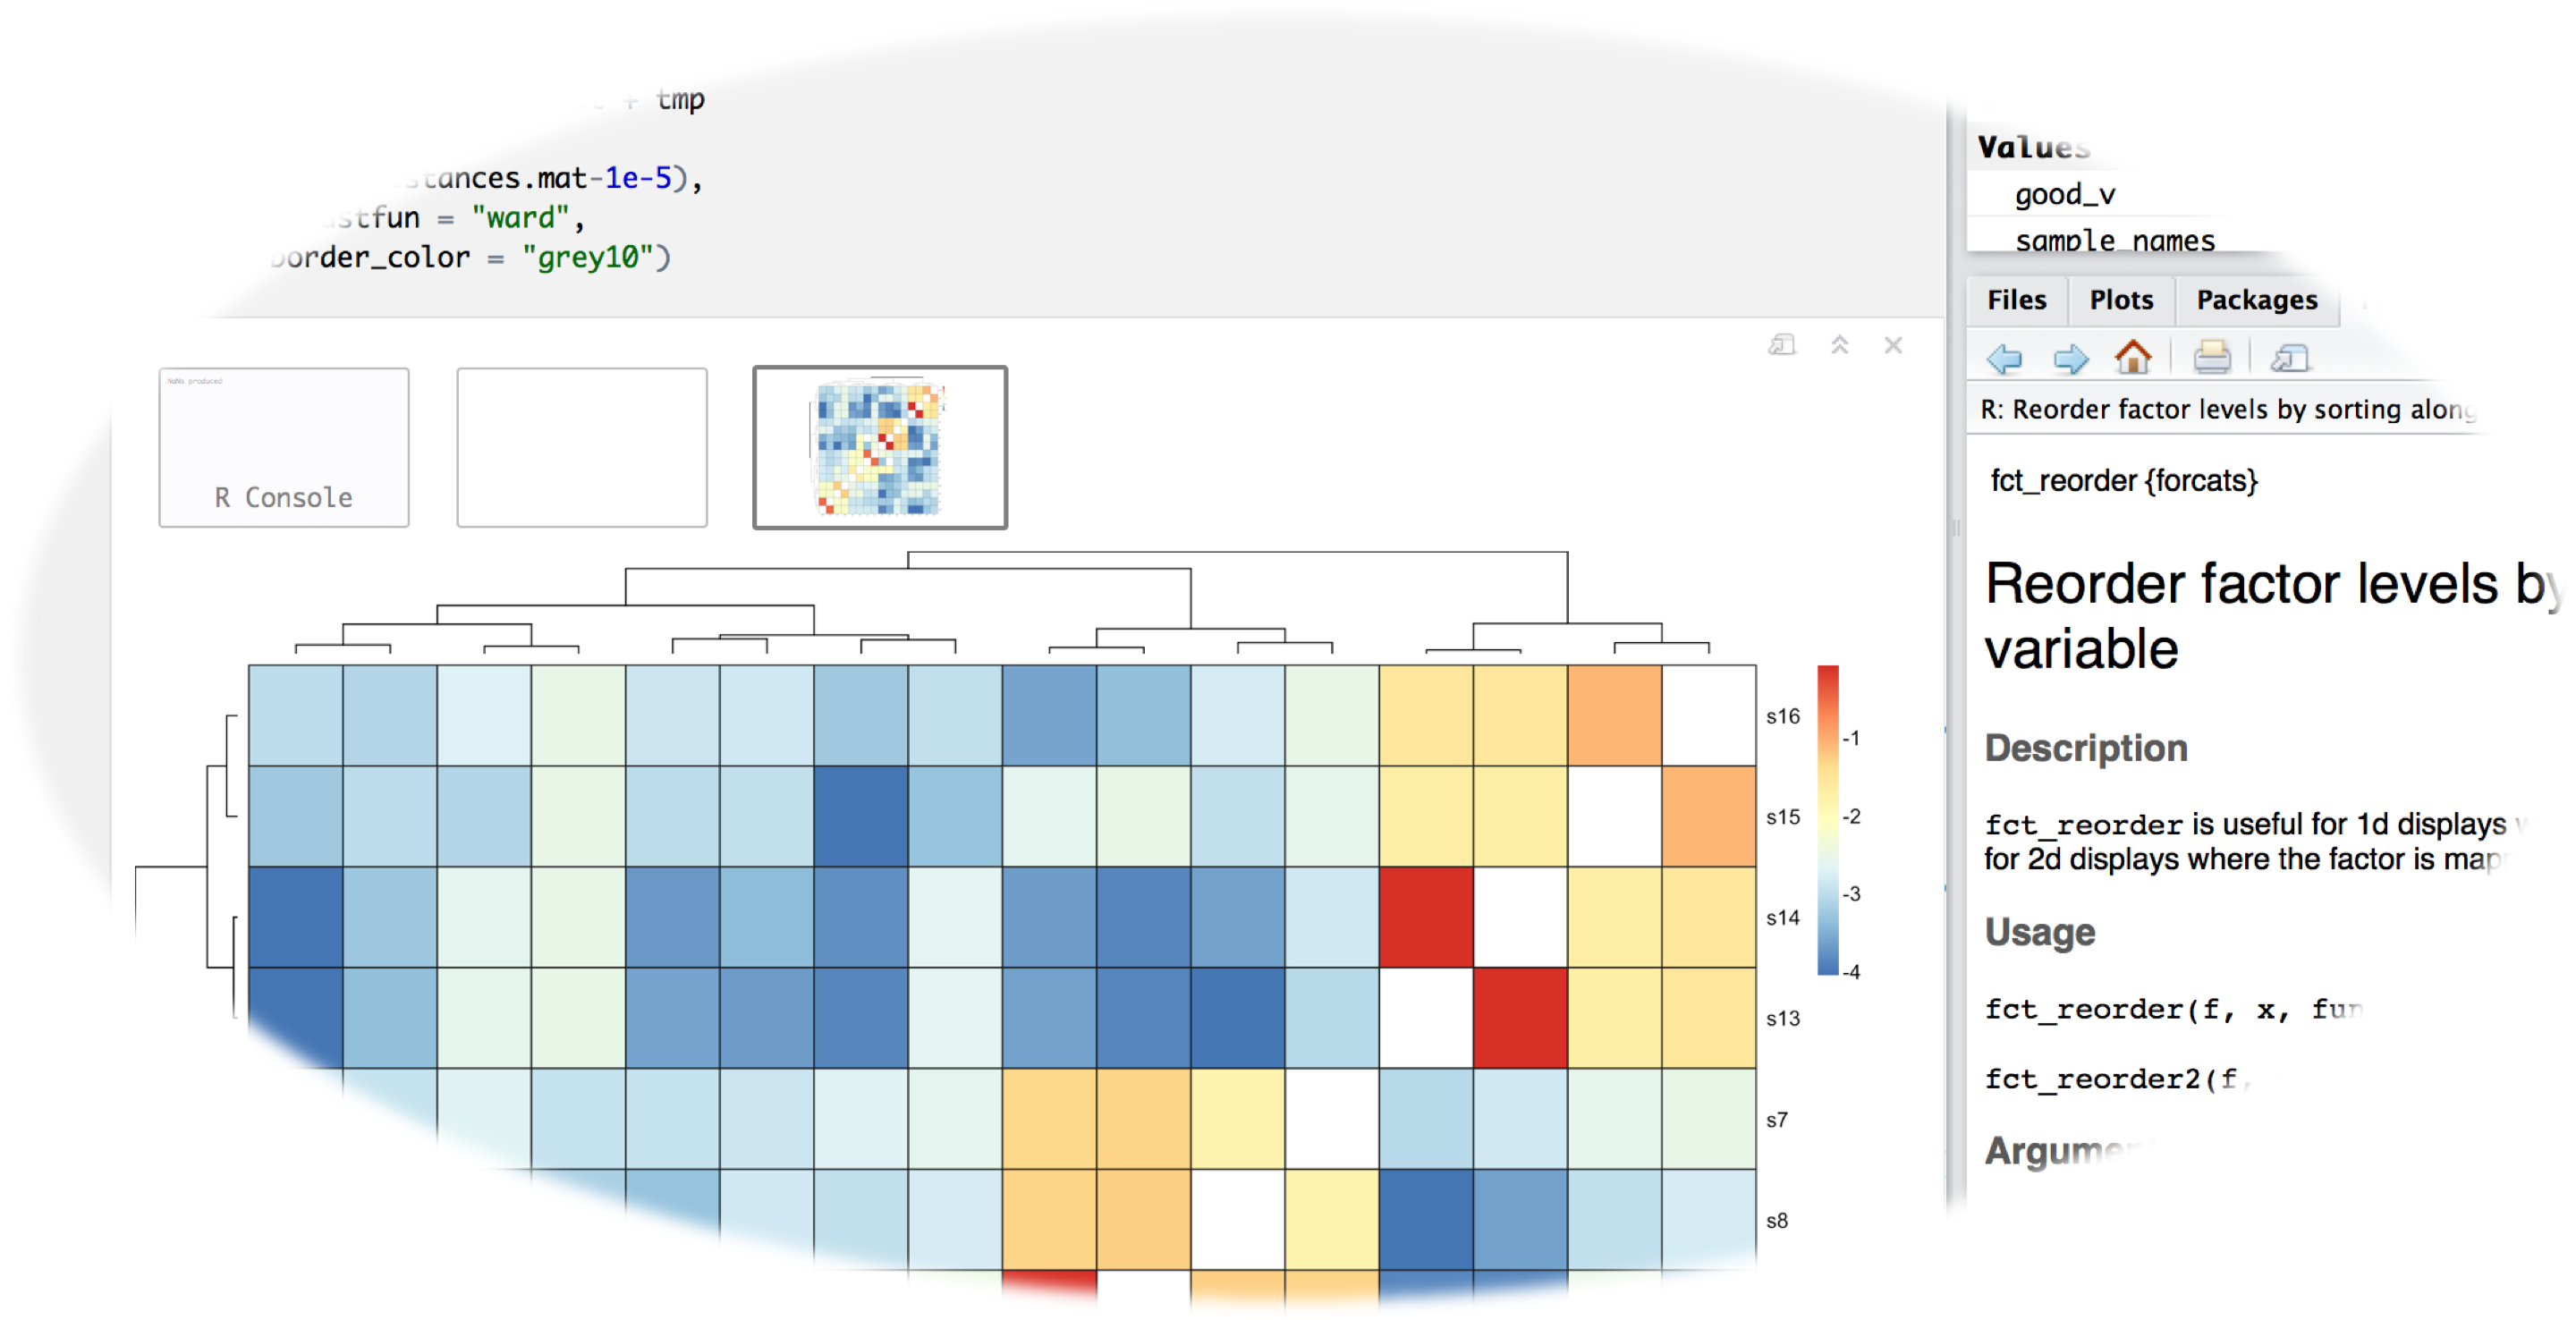
\includegraphics[width=\textwidth]{../splash}
\end{center}
\end{frame}

\section{The assignment}

\begin{frame}{...}
\end{frame}

\end{document}